\section{Comunicación TCP entre tres nodos}
\label{sec:tcp-jordan}

\subsection{Objetivo e hipótesis}

El objetivo fue implementar el intercambio de mensajes entre tres nodos por
sockets TCP y medir su latencia, throughput y comportamiento ante tres
solicitudes simultáneas. Como hipótesis previa, se esperaba que los relojes de
Lamport conservaran el orden causal de cada solicitud y su respuesta, y que
las mediciones variaran entre tamaños de mensaje bajo las mismas condiciones
locales. La dirección de esa variación no se presupuso.

La implementación TCP organiza la comunicación entre tres nodos, denominados
\texttt{nodo-A}, \texttt{nodo-B} y \texttt{nodo-C}. En la configuración
experimental, los tres se ejecutan en un mismo equipo y escuchan en la
dirección \texttt{127.0.0.1}, mediante los puertos 5000, 5001 y 5002,
respectivamente. Cada nodo puede iniciar solicitudes y atender las de los
otros. Esta disposición permite examinar el intercambio entre procesos sin
introducir las condiciones de una red entre equipos físicos.

\subsection{Arquitectura e intercambio de mensajes}

\begin{figure}[htbp]
\centering
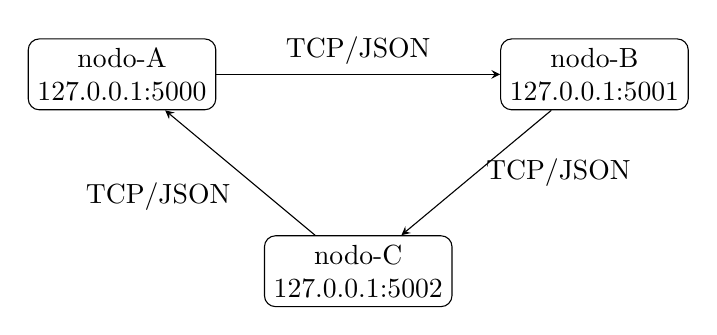
\begin{tikzpicture}[>=stealth]
\node[draw,rounded corners,align=center] (a) at (0,0) {nodo-A\\127.0.0.1:5000};
\node[draw,rounded corners,align=center] (b) at (6,0) {nodo-B\\127.0.0.1:5001};
\node[draw,rounded corners,align=center] (c) at (3,-2.5) {nodo-C\\127.0.0.1:5002};
\draw[->] (a) -- node[above]{TCP/JSON} (b);
\draw[->] (b) -- node[right]{TCP/JSON} (c);
\draw[->] (c) -- node[below left]{TCP/JSON} (a);
\end{tikzpicture}
\caption{Rutas de comunicación entre los tres nodos del experimento.}
\label{fig:arquitectura-tcp}
\end{figure}

El cliente establece una conexión con el puerto del nodo de destino mediante
un socket TCP. La solicitud se codifica en UTF-8 como una línea JSON con los
campos \texttt{sender}, \texttt{timestamp} y \texttt{message}. El servidor lee
esa línea, valida el emisor, el timestamp y el mensaje, y devuelve otra línea
JSON. En una respuesta válida se incluyen el nodo que respondió, el instante
lógico de recepción, el instante lógico de envío de la respuesta y un acuse
\texttt{ACK}. El servidor utiliza un manejador de solicitudes por conexión,
lo que permite atender comunicaciones simultáneas.

Cada nodo mantiene un reloj lógico de Lamport. Antes de enviar, incrementa su
contador y adjunta el nuevo valor a la solicitud. El receptor actualiza su
reloj al máximo entre su valor local y el recibido, más una unidad; antes de
responder vuelve a incrementarlo. Al recibir la respuesta, el cliente
actualiza también su reloj. Así, los cuatro instantes de un intercambio
válido siguen el orden envío del cliente, recepción del servidor, envío de la
respuesta y recepción del cliente. Los eventos de envío y recepción se
registran en archivos CSV por nodo con el tipo de evento, el valor lógico y
la hora real. El archivo \texttt{data/tcp\_exchanges.csv} conserva además
los cuatro timestamps de cada intercambio experimental.

Los registros TCP muestran, por ejemplo, un evento \texttt{receive} del
\texttt{nodo-A} con valor lógico 4 y un evento \texttt{send} del
\texttt{nodo-B} también con valor 4. La igualdad de valores entre nodos es
posible: el reloj de Lamport ordena eventos causales, pero un valor igual no
demuestra simultaneidad física ni basta por sí solo para establecer una
relación causal entre esos dos eventos.

\subsection{Procedimiento experimental}

Se realizaron 20 intercambios entre los nodos A y B, B y C, y C y A, en ese
orden de envío. Para medir la latencia de
solicitud y respuesta se emplearon mensajes de 100 y 10.240 bytes. Cada
tamaño tuvo una fase de calentamiento, seguida de cinco repeticiones de cien
mediciones; las muestras de calentamiento no forman parte del resumen. El
throughput de cada repetición se calculó como cien mensajes divididos por la
duración de ese lote. También se lanzaron tres solicitudes concurrentes, una
por cada ruta, mediante tres hilos sincronizados al inicio.

Las mediciones se guardaron en el archivo \texttt{tcp\_latency.csv} y las tres
observaciones concurrentes en \texttt{tcp\_concurrency.csv}, ambos dentro de
\texttt{data/}. El módulo \texttt{tcp\_statistics.py}, ubicado en
\texttt{analysis/}, agrupó las latencias por tamaño de
mensaje y calculó media, mediana, mínimo, máximo, desviación estándar
muestral, percentil 95 (P95) y promedio de los valores de throughput
registrados. El resumen se encuentra en \texttt{tcp\_statistics.csv} dentro
de \texttt{data/}.

\subsection{Resultados de TCP}

La Tabla~\ref{tab:tcp-jordan-estadisticas} presenta las métricas obtenidas
de las 500 muestras de cada tamaño. Todos los tiempos están expresados en
milisegundos; el throughput corresponde al promedio de la columna de
mensajes por segundo de los lotes experimentales.

\begin{table}[htbp]
\centering
\caption{Resumen estadístico de la latencia y el throughput TCP}
\label{tab:tcp-jordan-estadisticas}
\begin{tabular}{lrr}
\hline
\textbf{Métrica} & \textbf{100 bytes} & \textbf{10.240 bytes} \\
\hline
Muestras & 500 & 500 \\
Media (ms) & 7,220525 & 4,850986 \\
Mediana (ms) & 6,322050 & 4,079050 \\
Mínimo (ms) & 2,764400 & 2,937700 \\
Máximo (ms) & 31,517900 & 29,215500 \\
Desviación estándar (ms) & 3,797761 & 3,491191 \\
P95 (ms) & 13,501700 & 7,165695 \\
Throughput promedio (mensajes/s) & 144,301253 & 204,265171 \\
\hline
\end{tabular}
\end{table}

En esta ejecución, los mensajes de 10.240 bytes tuvieron una latencia media
menor que los de 100 bytes. La diferencia describe las mediciones obtenidas
en el equipo local y no establece por sí sola una relación general entre el
tamaño del mensaje y el rendimiento de TCP. Los máximos, superiores a las
respectivas medias, muestran además que hubo observaciones más lentas dentro
de ambas series.

La prueba concurrente produjo las tres latencias de la
Tabla~\ref{tab:tcp-jordan-concurrencia}. Estas cifras describen una única
ejecución con tres solicitudes simultáneas y no constituyen una medición
exhaustiva de escalabilidad.

\begin{table}[htbp]
\centering
\caption{Latencias registradas en la prueba concurrente TCP}
\label{tab:tcp-jordan-concurrencia}
\begin{tabular}{llr}
\hline
\textbf{Emisor} & \textbf{Destino} & \textbf{Latencia (ms)} \\
\hline
\texttt{nodo-A} & \texttt{nodo-B} & 6,1154 \\
\texttt{nodo-B} & \texttt{nodo-C} & 6,2118 \\
\texttt{nodo-C} & \texttt{nodo-A} & 6,6787 \\
\hline
\end{tabular}
\end{table}

Las pruebas se efectuaron sobre la interfaz local. Por ello, las latencias
incluyen el procesamiento y la comunicación entre procesos del mismo equipo,
pero no representan retardos de una red física entre computadoras.
